% arara: xelatex
% arara: biber
% arara: xelatex
% arara: xelatex

%%%%%%%%%%%%%%%%%%%%%%%%%%%%%%%%%%%%%%%%%
% CLASS OPTIONS
% language: czech/english/slovak
% thesis type: bachelor/master/dissertation
% colour: bw for black&white OR no option for default colour scheme
% electronic (oneside) or printed (twoside), twoside is default
% paragraph - if passed, this optional argument sets paragraphs as the deepest level of headers, styles it, numbers it and adds it to Table of Content. Use with care! Normally, it is considered unwise to use it, since its too deep.
%%%%%%%%%%%%%%%%%%%%%%%%%%%%%%%%%%%%%%%%%
\documentclass[english,bachelor,unicode,oneside]{ctufit-thesis}

%%%%%%%%%%%%%%%%%%%%%%%%%%%%%%%%%%
% FILL IN THIS INFORMATION
%%%%%%%%%%%%%%%%%%%%%%%%%%%%%%%%%%
\ctufittitle{TinyC Compiler Frontend}
\ctufitauthorfull{Mykhailo Anisimov}
\ctufitauthorsurnames{Anisimov} 
\ctufitauthorgivennames{Mykhailo}
\ctufitsupervisor{Ing.\,Petr Máj,\,Ph.D.}
\ctufitdepartment{Department of Software Engineering}
\ctufityear{2025}
\ctufitdeclarationplace{Prague}
\ctufitdeclarationdate{\today}
\ctufitabstractCZE{Fill in the abstract of this thesis in Czech. Lorem ipsum dolor sit amet. Class aptent taciti sociosqu ad litora torquent per conubia nostra, per inceptos hymenaeos. Cras pede libero, dapibus nec, pretium sit amet, tempor quis. Sed vel lectus. Donec odio tempus molestie, porttitor ut, iaculis quis, sem. Suspendisse sagittis ultrices augue.}
\ctufitabstractENG{Fill in the abstract of this thesis in English. Lorem ipsum dolor sit amet. Class aptent taciti sociosqu ad litora torquent per conubia nostra, per inceptos hymenaeos. Cras pede libero, dapibus nec, pretium sit amet, tempor quis. Sed vel lectus. Donec odio tempus molestie, porttitor ut, iaculis quis, sem. Suspendisse sagittis ultrices augue.}
\ctufitkeywordsCZE{enter, comma, separated, list, of, keywords, in, CZECH}
\ctufitkeywordsENG{enter, comma, separated, list, of, keywords, in, ENGLISH}
%%%%%%%%%%%%%%%%%%%%%%%%%%%%%%%%%%
% END FILL IN
%%%%%%%%%%%%%%%%%%%%%%%%%%%%%%%%%%

%%%%%%%%%%%%%%%%%%%%%%%%%%%%%%%%%%
% CUSTOMIZATION of this template
% Skip this part or alter it if you know what you are doing.
%%%%%%%%%%%%%%%%%%%%%%%%%%%%%%%%%%

\RequirePackage{iftex}[2020/03/06]
\iftutex % XeLaTeX and LuaLaTeX
    \RequirePackage{ellipsis}[2020/05/22] %ellipsis workaround for XeLaTeX
\else
    \errmessage{Only compilation with XeLaTeX or LuaLaTeX is allowed}
    \stop
\fi

% hyperlinks
\hypersetup{
    pdfpagelayout=TwoPageRight,
    colorlinks=false,
    allcolors=decoration,
    pdfborder={0 0 0.1}
}

% uncomment the following to hide all hyperlinks
%\hypersetup{hidelinks}

% uncomment the following to change the colour of all hyperlinks to CTU blue
%\hypersetup{allbordercolors=decoration}

\RequirePackage{pdfpages}[2020/01/28]

%%%%%%%%%%%%%%%%%%%%%%%%%%%%%%%%%%
% CUSTOMIZATION of this template END
%%%%%%%%%%%%%%%%%%%%%%%%%%%%%%%%%%


%%%%%%%%%%%%%%%%%%%%%%
% DEMO CONTENTS SETTINGS
% You may choose to modify this part.
%%%%%%%%%%%%%%%%%%%%%%
\usepackage{dirtree}
\usepackage{lipsum,tikz}
\usepackage[style=iso-numeric]{biblatex}
\addbibresource{text/bib-database.bib}
\usepackage{xurl}
\usepackage{listings} % typesetting of sources
\usepackage{syntax}

% \usepackage{minted}


\usepackage{csquotes}


% Custom commands below
\usepackage{amsmath}
\allowdisplaybreaks    % Allows align/alignat to break across pages if needed


%%%%%%%%%%%%%%%%%%%%%%
% DEMO CONTENTS SETTINGS END
%%%%%%%%%%%%%%%%%%%%%%
\begin{document}
\frontmatter\frontmatterinit % do not remove these two commands

\thispagestyle{empty}\maketitle\thispagestyle{empty}\cleardoublepage % do not remove these four commands

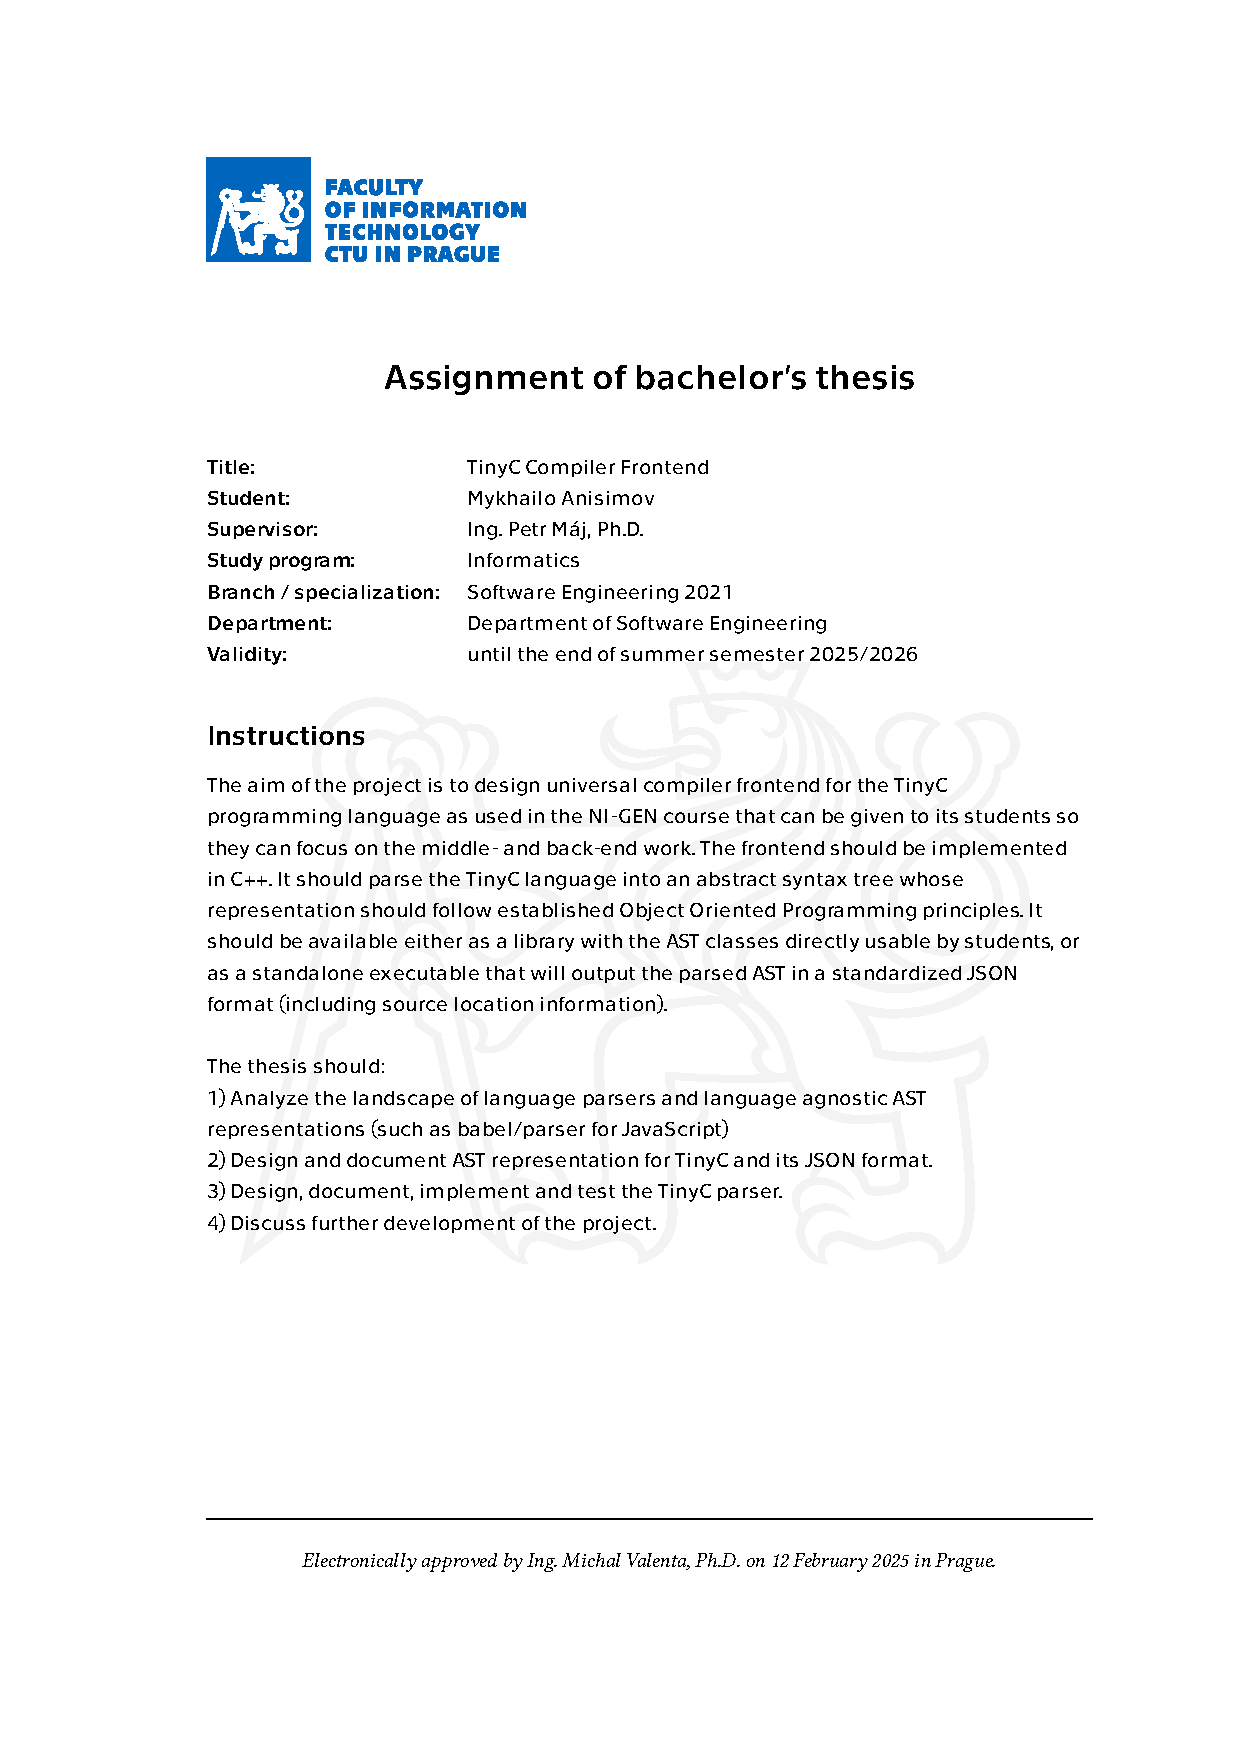
\includepdf[pages={1-}]{Assignment.pdf} % replace this file with your thesis assignment generated from ProjectsFIT

\imprintpage % do not remove this command
\stopTOCentries
%%%%%%%%%%%%%%%%%%%%%%
% list of other contents END
%%%%%%%%%%%%%%%%%%%%%%

%%%%%%%%%%%%%%%%%%%
% ACKNOWLEDGMENT
% FILL IN / MODIFY
% This is a place to thank people for helping you. It is common to thank your supervisor.
%%%%%%%%%%%%%%%%%%%
\begin{acknowledgmentpage}
	Here goes the acknowledgment part...
\end{acknowledgmentpage} 
%%%%%%%%%%%%%%%%%%%
% ACKNOWLEDGMENT END
%%%%%%%%%%%%%%%%%%%


%%%%%%%%%%%%%%%%%%%
% DECLARATION
% FILL IN / MODIFY
%%%%%%%%%%%%%%%%%%%
% INSTRUCTIONS
% ENG: choose one of approved texts of the declaration. DO NOT CREATE YOUR OWN. Find the approved texts at https://courses.fit.cvut.cz/SFE/download/index.html#_documents (document Declaration for FT in English)
% CZE/SLO: Vyberte jedno z fakultou schvalenych prohlaseni. NEVKLADEJTE VLASTNI TEXT. Schvalena prohlaseni najdete zde: https://courses.fit.cvut.cz/SZZ/dokumenty/index.html#_dokumenty (prohlášení do ZP)
\begin{declarationpage}
FILL IN ACCORDING TO THE INSTRUCTIONS. VYPLŇTE V SOULADU S POKYNY. Lorem ipsum dolor sit amet, consectetuer adipiscing elit. Curabitur sagittis hendrerit ante. Class aptent taciti sociosqu ad litora torquent per conubia nostra, per inceptos hymenaeos. Cras pede libero, dapibus nec, pretium sit amet, tempor quis. Sed vel lectus. Donec odio tempus molestie, porttitor ut, iaculis quis, sem. Suspendisse sagittis ultrices augue. Donec ipsum massa, ullamcorper in, auctor et, scelerisque sed, est. In sem justo, commodo ut, suscipit at, pharetra vitae, orci. Pellentesque pretium lectus id turpis.

Lorem ipsum dolor sit amet, consectetuer adipiscing elit. Curabitur sagittis hendrerit ante. Class aptent taciti sociosqu ad litora torquent per conubia nostra, per inceptos hymenaeos. Cras pede libero, dapibus nec, pretium sit amet, tempor quis. Sed vel lectus. Donec odio tempus molestie, porttitor ut, iaculis quis, sem. Suspendisse sagittis ultrices augue. Donec ipsum massa, ullamcorper in, auctor et, scelerisque sed, est. In sem justo, commodo ut, suscipit at, pharetra vitae, orci. Pellentesque pretium lectus id turpis.
\end{declarationpage}
%%%%%%%%%%%%%%%%%%%
% DECLARATION END
%%%%%%%%%%%%%%%%%%%

\printabstractpage % do not remove this command

%%%%%%%%%%%%%%%%%%%
% SUMMARY
% FILL IN / MODIFY
% OR REMOVE ENTIRELY (upon agreement with your supervisor)
% (appropriate to remove in most theses)
%%%%%%%%%%%%%%%%%%%
% \begin{summarypage}
% \section*{Summary section}
% 
% \lipsum[1][1-8]
% 
% \section*{Summary section}
% 
% \lipsum[2][1-6]
% 
% \section*{Summary section}
% 
% \lipsum[3]
% 
% \section*{Summary section}
% 
% \lipsum[2]
% 
% \section*{Summary section}
% 
% \lipsum[1][1-8] Lorem lorem lorem.
% \end{summarypage}
%%%%%%%%%%%%%%%%%%%
% SUMMARY END
%%%%%%%%%%%%%%%%%%%

\tableofcontents % do not remove this command
%%%%%%%%%%%%%%%%%%%%%%
% list of other contents: figures, tables, code listings, algorithms, etc.
% add/remove commands accordingly
%%%%%%%%%%%%%%%%%%%%%%
\listoffigures % list of figures
\begingroup
\let\clearpage\relax
\listoftables % list of tables
\thectufitlistingscommand
\endgroup

%%%%%%%%%%%%%%%%%%%
% ABBREVIATIONS
% FILL IN / MODIFY
% OR REMOVE ENTIRELY
% List the abbreviations in lexicography order.
%%%%%%%%%%%%%%%%%%%
\chapter{\thectufitabbreviationlabel}
	
\begin{tabular}{rl}
DFA & Deterministic Finite Automaton\\
FA & Finite Automaton\\
LPS & Labelled Prüfer Sequence\\
NFA & Nondeterministic Finite Automaton\\
NPS & Numbered Prüfer Sequence\\
XML & Extensible Markup Language\\
XPath & XML Path Language\\
XSLT & eXtensible Stylesheet Language Transformations\\
W3C & World Wide Web Consortium
\end{tabular}
%%%%%%%%%%%%%%%%%%%
% ABBREVIATIONS END
%%%%%%%%%%%%%%%%%%%
\resumeTOCentries
\mainmatter\mainmatterinit % do not remove these two commands
%%%%%%%%%%%%%%%%%%%
% THE THESIS
% MODIFY ANYTHING BELOW THIS LINE
%%%%%%%%%%%%%%%%%%%

\chapter{2nd exercise}

Each (sub)chapter should have some introductory text.

\section{Microtypography}

A text -- especially a professional one such as this work - must be divided into paragraphs. Each paragraph should relate to one topic or idea\dots{} Paragraphs must be visually separated from each other. There are several suitable styles for this, which we described in  the last lecture. Paragraphs can be set in different ways. In professional texts, the ``block'' typesetting is common. It is necessary to change the interword spaces appropriately. Their recommended size is 0.25--0.33 square.


\section{Source code}

The main part of our program's operation can be found in Listing~\ref{code:cpp}. It is worth noting that the main function has a return type of int, which is, of course, very atypical, and therefore, it is worth documenting. We will only include code samples in the work when it really brings something new, not just for the sake of having a code sample.

\begin{listing}
    \begin{minted}{c++}
#include<iostream>

using namespace std;

int main()
{
    cout << "Hello, world!" << endl;
    return 0;
}
    \end{minted}
    \caption{The main function of our program}
    \label{code:cpp}
\end{listing}

\section{Tables}

% In Table 3.1, you will find options for earning points in the BI-TDP subject. Although it's not as good a table as the chocolate table, it will have to be enough for us to get credit. I'm not saying that you should bribe your students with chocolate bars! But I'm also not saying that you shouldn't.

% Graded activities in TDP

% activity | points | mandatory
% Processing and submitting a credit project (bachelor's thesis in progress) | 30 | YES
% Typography test | 10 | YES
% Citation test | 10 | YES
% Awarding points from the thesis supervisor | 20 | NO

% \begin{table}[ht]
% \centering
% \begin{tabular}{|c|c|}
% \hline
% This text will be too long and will not fit on one line. & This text will be too long and will not fit on one line. \\\hline
% This text will be too long and will not fit on one line. & This text will be too long and will not fit on one line. \\\hline
% \end{tabular}
% \caption{Caption}
% \label{tab:wideTable}
% \end{table}

% \begin{tabular}{|c|c|}
% \hline
% \textbf{Heading 1} & \textbf{Heading 2}\\ \hline
% data & text\\\hline
% data & text\\\hline
% data & text\\\hline
% data & text\\\hline
% data & text\\\hline
% data & text\\\hline
% data & text\\\hline
% data & text\\\hline
% data & text\\\hline
% data & text\\\hline
% data & text\\\hline
% data & text\\\hline
% data & text\\\hline
% data & text\\\hline
% data & text\\\hline
% data & text\\\hline
% data & text\\\hline
% data & text\\\hline
% data & text\\\hline
% data & text\\\hline
% data & text\\\hline
% data & text\\\hline
% data & text\\\hline
% data & text\\\hline
% data & text\\\hline
% data & text\\\hline
% data & text\\\hline
% data & text\\\hline
% data & text\\\hline
% data & text\\\hline
% data & text\\\hline
% data & text\\\hline
% data & text\\\hline
% data & text\\\hline
% data & text\\\hline
% data & text\\\hline
% data & text\\\hline
% data & text\\\hline
% data & text\\\hline
% data & text\\\hline
% data & text\\\hline
% data & text\\\hline
% data & text\\\hline
% data & text\\\hline
% data & text\\\hline
% data & text\\\hline
% data & text\\\hline
% data & text\\\hline
% data & text\\\hline
% data & text\\\hline
% data & text\\\hline
% data & text\\\hline
% data & text\\\hline
% data & text\\\hline
% data & text\\\hline
% data & text\\\hline
% data & text\\\hline
% data & text\\\hline
% data & text\\\hline
% data & text\\\hline
% data & text\\\hline
% data & text\\\hline
% data & text\\\hline
% data & text\\\hline
% data & text\\\hline
% data & text\\\hline
% data & text\\\hline
% data & text\\\hline
% data & text\\\hline
% data & text\\\hline
% data & text\\\hline
% data & text\\\hline
% data & text\\\hline
% data & text\\\hline
% data & text\\\hline
% data & text\\\hline
% data & text\\\hline
% data & text\\\hline
% data & text\\\hline
% data & text\\\hline
% data & text\\\hline
% data & text\\\hline
% data & text\\\hline
% data & text\\\hline
% data & text\\\hline
% data & text\\\hline
% data & text\\\hline
% data & text\\\hline
% data & text\\\hline
% data & text\\\hline
% data & text\\\hline
% data & text\\\hline
% data & text\\\hline
% data & text\\\hline
% data & text\\\hline
% \end{tabular}

 % include `text.tex' from `text/' subdirectory

\appendix\appendixinit % do not remove these two commands

\chapter{TinyC Grammar}


\section{Program and Program Items}
\begin{align*}
\text{PROGRAM}
  &\to \text{PROGRAM\_ITEM}\;\text{PROGRAM}\\
  &\to \varepsilon\\[6pt]
\text{PROGRAM\_ITEM}
  &\to \text{TYPE\_FUN\_RET}\;\text{identifier}\;\text{PROGRAM\_ITEM\_TAIL}\\
  &\to \text{STRUCT\_DECL}\\
  &\to \text{FUNPTR\_DECL}\\[6pt]
\text{PROGRAM\_ITEM\_TAIL}
  &\to (\,\text{OPT\_FUN\_ARGS}\,)\;\text{FUNC\_TAIL}\\
  &\to \text{GLOBAL\_VAR\_TAIL}\; ;\\[6pt]
\text{FUNC\_TAIL}
  &\to \text{BLOCK\_STMT}\\
  &\to ;
\end{align*}

\begin{align*}
\text{GLOBAL\_VAR\_TAIL}
  &\to \text{OPT\_ARRAY\_SIZE}\;\text{OPT\_INIT}\;\text{MORE\_GLOBAL\_VARS}\\[6pt]
\text{MORE\_GLOBAL\_VARS}
  &\to ,\;\text{identifier}\;\text{OPT\_ARRAY\_SIZE}\;\text{OPT\_INIT}\;\text{MORE\_GLOBAL\_VARS}\\
  &\to \varepsilon\\[6pt]
\text{OPT\_FUN\_ARGS}
  &\to \text{FUN\_ARG}\;\text{FUN\_ARG\_TAIL}\\
  &\to \varepsilon\\[6pt]
\text{FUN\_ARG\_TAIL}
  &\to ,\;\text{FUN\_ARG}\;\text{FUN\_ARG\_TAIL}\\
  &\to \varepsilon\\[6pt]
\text{FUN\_ARG}
  &\to \text{TYPE}\;\text{identifier}
\end{align*}

%----------------------------------------
\section{Statements}
\begin{align*}
\text{STATEMENT}
  &\to \text{BLOCK\_STMT}\\
  &\to \text{IF\_STMT}\\
  &\to \text{SWITCH\_STMT}\\
  &\to \text{WHILE\_STMT}\\
  &\to \text{DO\_WHILE\_STMT}\\
  &\to \text{FOR\_STMT}\\
  &\to \text{BREAK\_STMT}\\
  &\to \text{CONTINUE\_STMT}\\
  &\to \text{RETURN\_STMT}\\
  &\to \text{EXPR\_STMT}\\[6pt]
\text{BLOCK\_STMT}
  &\to \{\,\text{STATEMENT\_STAR}\,\}\\[6pt]
\text{STATEMENT\_STAR}
  &\to \text{STATEMENT}\;\text{STATEMENT\_STAR}\\
  &\to \varepsilon
\end{align*}

\begin{align*}
\text{IF\_STMT}
  &\to \text{if}\;(\,\text{EXPR}\,)\;\{\,\text{STATEMENT}\}\;\text{ELSE\_PART}\\[6pt]
\text{ELSE\_PART}
  &\to \text{else}\;\text{STATEMENT}\\
  &\to \varepsilon\\[6pt]
\text{SWITCH\_STMT}
  &\to \text{switch}\;(\,\text{EXPR}\,)\;\{\,\text{CASE\_WITH\_DEFAULT\_STMT\_STAR}\}\\[6pt]
\text{CASE\_WITH\_DEFAULT\_STMT\_STAR}
  &\to \text{CASE\_STMT}\;\text{CASE\_WITH\_DEFAULT\_STMT\_STAR}\\
  &\to \varepsilon\\
  &\to \text{DEFAULT\_CASE}\;\text{CASE\_STMT\_STAR}\\[6pt]
\text{CASE\_STMT\_STAR}
  &\to \text{CASE\_STMT}\;\text{CASE\_STMT\_STAR}\\
  &\to \varepsilon\\[6pt]
\text{CASE\_STMT}
  &\to \text{case}\;\text{integer\_literal}\;:\;\text{CASE\_BODY}\\[6pt]
\text{CASE\_BODY}
  &\to \text{STATEMENT\_STAR}\\[6pt]
\text{DEFAULT\_CASE}
  &\to \text{default}\;:\;\text{CASE\_BODY}
\end{align*}

\begin{align*}
\text{WHILE\_STMT}
  &\to \text{while}\;(\,\text{EXPR}\,)\;\text{STATEMENT}\\[6pt]
\text{DO\_WHILE\_STMT}
  &\to \text{do}\;\text{STATEMENT}\;\text{while}\;(\,\text{EXPR}\,)\; ;\\[6pt]
\text{FOR\_STMT}
  &\to \text{for}\;( \text{OPT\_EXPR\_OR\_VAR\_DECL}\; ;\; \text{OPT\_EXPR}\; ;\; \text{OPT\_EXPR} )\;\text{STATEMENT}\\[6pt]
\text{OPT\_EXPR\_OR\_VAR\_DECL}
  &\to \text{EXPR\_OR\_VAR\_DECL}\\
  &\to \varepsilon\\[6pt]
\text{OPT\_EXPR}
  &\to \text{EXPR}\\
  &\to \varepsilon
\end{align*}

\begin{align*}
\text{BREAK\_STMT}
  &\to \text{break}\; ;\\[6pt]
\text{CONTINUE\_STMT}
  &\to \text{continue}\; ;\\[6pt]
\text{RETURN\_STMT}
  &\to \text{return}\;\text{OPT\_EXPR}\; ;\\[6pt]
\text{EXPR\_STMT}
  &\to \text{EXPR\_OR\_VAR\_DECL}\; ;
\end{align*}

%----------------------------------------
\section{Expression or Variable Declarations}
\begin{align*}
\text{EXPR\_OR\_VAR\_DECL}
  &\to \text{VAR\_DECLS}\\
  &\to \text{EXPRS}\\[6pt]
\text{VAR\_DECLS}
  &\to \text{VAR\_DECL}\;\text{VAR\_DECLS\_TAIL}\\[6pt]
\text{VAR\_DECLS\_TAIL}
  &\to ,\;\text{VAR\_DECL}\;\text{VAR\_DECLS\_TAIL}\\
  &\to \varepsilon\\[6pt]
\text{VAR\_DECL}
  &\to \text{TYPE}\;\text{identifier}\;\text{OPT\_ARRAY\_SIZE}\;\text{OPT\_INIT}\\[6pt]
\text{OPT\_ARRAY\_SIZE}
  &\to [\;\text{E9}\;]\\
  &\to \varepsilon\\[6pt]
\text{OPT\_INIT}
  &\to =\;\text{EXPR}\\
  &\to \varepsilon
\end{align*}

\begin{align*}
\text{EXPRS}
  &\to \text{EXPR}\;\text{EXPRS\_TAIL}\\[6pt]
\text{EXPRS\_TAIL}
  &\to ,\;\text{EXPR}\;\text{EXPRS\_TAIL}\\
  &\to \varepsilon
\end{align*}

%----------------------------------------
\section{Types}
\begin{align*}
\text{TYPE\_FUN\_RET}
  &\to \text{BaseOrIdType}\\
  &\to \text{void}\;\text{TypeFunRetTail}\\[6pt]
\text{BaseOrIdType}
  &\to \text{BASE\_TYPE}\;\text{STAR\_SEQ}\\
  &\to \text{TYPENAME}\;\text{STAR\_SEQ}\\[6pt]
\text{TypeFunRetTail}
  &\to \text{STAR\_PLUS}\\
  &\to \varepsilon\\[6pt]
\text{TYPE}
  &\to \text{BaseOrIdType}\\
  &\to \text{void}\;\text{STAR\_PLUS}\\[6pt]
\text{BASE\_TYPE}
  &\to \text{int}\\
  &\to \text{double}\\
  &\to \text{char}\\[6pt]
\text{STAR\_PLUS}
  &\to *\;\text{STAR\_SEQ}\\[6pt]
\text{STAR\_SEQ}
  &\to *\;\text{STAR\_SEQ}\\
  &\to \varepsilon
\end{align*}

%----------------------------------------
\section{Struct Declarations}
\begin{align*}
\text{STRUCT\_DECL}
  &\to \text{struct}\;\text{identifier}\;\text{OPT\_STRUCT\_BODY}\; ;\\[6pt]
\text{OPT\_STRUCT\_BODY}
  &\to \{\,\text{STRUCT\_FIELDS}\,\}\\
  &\to \varepsilon\\[6pt]
\text{STRUCT\_FIELDS}
  &\to \text{STRUCT\_FIELD}\;\text{STRUCT\_FIELDS}\\
  &\to \varepsilon\\[6pt]
\text{STRUCT\_FIELD}
  &\to \text{TYPE}\;\text{identifier}\; ;
\end{align*}

%----------------------------------------
\section{Function Pointer Declarations}
\begin{align*}
\text{FUNPTR\_DECL}
  &\to \text{typedef}\;\text{TYPE\_FUN\_RET}\;( *\;\text{identifier} )(\,\text{OPT\_FUNPTR\_ARGS}\,)\; ;\\[6pt]
\text{OPT\_FUNPTR\_ARGS}
  &\to \text{FUNPTR\_ARGS}\\
  &\to \varepsilon\\[6pt]
\text{FUNPTR\_ARGS}
  &\to \text{TYPE}\;\text{FUNPTR\_ARGS\_TAIL}\\[6pt]
\text{FUNPTR\_ARGS\_TAIL}
  &\to ,\;\text{TYPE}\;\text{FUNPTR\_ARGS\_TAIL}\\
  &\to \varepsilon
\end{align*}

%----------------------------------------
\section{Expressions}
\begin{align*}
\text{EXPR}
  &\to \text{E9}\;\text{EXPR\_TAIL}\\[6pt]
\text{EXPR\_TAIL}
  &\to =\;\text{EXPR}\\
  &\to \varepsilon
\end{align*}

\begin{align*}
\text{E9}
  &\to \text{E8}\;\text{E9\_Prime}\\[6pt]
\text{E9\_Prime}
  &\to ||\;\text{E8}\;\text{E9\_Prime}\\
  &\to \varepsilon
\end{align*}

\begin{align*}
\text{E8}
  &\to \text{E7}\;\text{E8\_Prime}\\[6pt]
\text{E8\_Prime}
  &\to &&\;\text{E7}\;\text{E8\_Prime}\\
  &\to \varepsilon
\end{align*}

\begin{align*}
\text{E7}
  &\to \text{E6}\;\text{E7\_Prime}\\[6pt]
\text{E7\_Prime}
  &\to |\;\text{E6}\;\text{E7\_Prime}\\
  &\to \varepsilon
\end{align*}

\begin{align*}
\text{E6}
  &\to \text{E5}\;\text{E6\_Prime}\\[6pt]
\text{E6\_Prime}
  &\to &\;\text{E5}\;\text{E6\_Prime}\\
  &\to \varepsilon
\end{align*}

\begin{align*}
\text{E5}
  &\to \text{E4}\;\text{E5\_Prime}\\[6pt]
\text{E5\_Prime}
  &\to ==\;\text{E4}\;\text{E5\_Prime}\\
  &\to !=\;\text{E4}\;\text{E5\_Prime}\\
  &\to \varepsilon
\end{align*}

\begin{align*}
\text{E4}
  &\to \text{E3}\;\text{E4\_Prime}\\[6pt]
\text{E4\_Prime}
  &\to <\;\text{E3}\;\text{E4\_Prime}\\
  &\to <=\;\text{E3}\;\text{E4\_Prime}\\
  &\to >\;\text{E3}\;\text{E4\_Prime}\\
  &\to >=\;\text{E3}\;\text{E4\_Prime}\\
  &\to \varepsilon
\end{align*}

\begin{align*}
\text{E3}
  &\to \text{E2}\;\text{E3\_Prime}\\[6pt]
\text{E3\_Prime}
  &\to <<\;\text{E2}\;\text{E3\_Prime}\\
  &\to >>\;\text{E2}\;\text{E3\_Prime}\\
  &\to \varepsilon
\end{align*}

\begin{align*}
\text{E2}
  &\to \text{E1}\;\text{E2\_Prime}\\[6pt]
\text{E2\_Prime}
  &\to +\;\text{E1}\;\text{E2\_Prime}\\
  &\to -\;\text{E1}\;\text{E2\_Prime}\\
  &\to \varepsilon
\end{align*}

\begin{align*}
\text{E1}
  &\to \text{E\_UNARY\_PRE}\;\text{E1\_Prime}\\[6pt]
\text{E1\_Prime}
  &\to *\;\text{E\_UNARY\_PRE}\;\text{E1\_Prime}\\
  &\to /\;\text{E\_UNARY\_PRE}\;\text{E1\_Prime}\\
  &\to %\;\text{E\_UNARY\_PRE}\;\text{E1\_Prime}\\
  &\to \varepsilon
\end{align*}

\begin{align*}
\text{E\_UNARY\_PRE}
  &\to +\;\text{E\_UNARY\_PRE}\\
  &\to -\;\text{E\_UNARY\_PRE}\\
  &\to !\;\text{E\_UNARY\_PRE}\\
  &\to \sim\;\text{E\_UNARY\_PRE}\\
  &\to ++\;\text{E\_UNARY\_PRE}\\
  &\to --\;\text{E\_UNARY\_PRE}\\
  &\to *\;\text{E\_UNARY\_PRE}\\
  &\to &\;\text{E\_UNARY\_PRE}\\
  &\to \text{E\_CALL\_INDEX\_MEMBER\_POST}
\end{align*}

\begin{align*}
\text{E\_CALL\_INDEX\_MEMBER\_POST}
  &\to \text{F}\;\text{E\_CALL\_INDEX\_MEMBER\_POST\_Prime}\\[6pt]
\text{E\_CALL\_INDEX\_MEMBER\_POST\_Prime}
  &\to \text{E\_CALL}\;\text{E\_CALL\_INDEX\_MEMBER\_POST\_Prime}\\
  &\to \text{E\_INDEX}\;\text{E\_CALL\_INDEX\_MEMBER\_POST\_Prime}\\
  &\to \text{E\_MEMBER}\;\text{E\_CALL\_INDEX\_MEMBER\_POST\_Prime}\\
  &\to \text{E\_POST}\;\text{E\_CALL\_INDEX\_MEMBER\_POST\_Prime}\\
  &\to \varepsilon
\end{align*}

\begin{align*}
\text{E\_CALL}
  &\to (\;\text{OPT\_EXPR\_LIST}\;)\\[6pt]
\text{OPT\_EXPR\_LIST}
  &\to \text{EXPR}\;\text{EXPR\_TAIL\_LIST}\\
  &\to \varepsilon\\[6pt]
\text{EXPR\_TAIL\_LIST}
  &\to ,\;\text{EXPR}\;\text{EXPR\_TAIL\_LIST}\\
  &\to \varepsilon
\end{align*}

\begin{align*}
\text{E\_INDEX}
  &\to [\;\text{EXPR}\;]\\[6pt]
\text{E\_MEMBER}
  &\to .\;\text{identifier}\\
  &\to \sim>\;\text{identifier}\\[6pt]
\text{E\_POST}
  &\to ++\\
  &\to --
\end{align*}

\begin{align*}
\text{F}
  &\to \text{integer\_literal}\\
  &\to \text{double\_literal}\\
  &\to \text{char\_literal}\\
  &\to \text{string\_literal}\\
  &\to \text{identifier}\\
  &\to (\;\text{EXPR}\;)\\
  &\to \text{E\_CAST}\\[6pt]
\text{E\_CAST}
  &\to \text{cast}\;<\;\text{TYPE}\;>\;(\;\text{EXPR}\;)
\end{align*}
 % include `appendix.tex' from `text/' subdirectory

\backmatter % do not remove this command

\printbibliography % print out the BibLaTeX-generated bibliography list

\chapter{Contents of the attachments}
% Contents of the attachment

	\dirtree{%
		.1 /.
		.2 readme.txt\DTcomment{stručný popis obsahu média}.
		.2 exe\DTcomment{adresář se spustitelnou formou implementace}.
		.2 src.
		.3 impl\DTcomment{zdrojové kódy implementace}.
		.3 thesis\DTcomment{zdrojová forma práce ve formátu \LaTeX{}}.
		.2 text\DTcomment{text práce}.
		.3 thesis.pdf\DTcomment{text práce ve formátu PDF}.
	}
 % include `medium.tex' from `text/' subdirectory

\end{document}
